% ============================================================
% Reporte: datapath-1
% Generado a partir de reportes/comun/plantilla_base.tex
% (NO edites la plantilla: cada unidad trabaja en su main.tex)
%
% Reglas de secciones y extensiones: reportes/AGENTS.md
% Compilar SIEMPRE con:
%   ../../scripts/latexbuild main.tex      (desde esta carpeta)
%   → genera build/main.pdf
% ============================================================
\documentclass[llncs]{llncs}

\usepackage[utf8]{inputenc}
\usepackage[T1]{fontenc}
\usepackage{fontspec}
\setmonofont{DejaVu Sans Mono}
\usepackage{graphicx}
\usepackage{amsmath}
\usepackage{tikz}
\usetikzlibrary{arrows.meta,positioning}
\usepackage{listings}
\usepackage{hyperref}
\usepackage{xcolor}

% ---- Estilo para código VHDL (apéndice y fragmentos) ----
\lstdefinestyle{vhdl}{
  language=VHDL,
  basicstyle=\ttfamily\scriptsize,
  keywordstyle=\color{black},
  commentstyle=\color{gray}\itshape,
  stringstyle=\color{black},
  showstringspaces=false,
  breaklines=true,
  frame=single,
  rulecolor=\color{black}
}
\lstset{style=vhdl}
\setlength{\emergencystretch}{2em}

\begin{document}

% ============================================================
% TÍTULO Y AUTORES  (rellenar: los 5 integrantes del equipo)
% ============================================================
% TODO título provisional: pendiente de validación por el equipo
\title{Diseño y Verificación de un Datapath con MUX, ALU y Registro Realimentado en {VHDL}}

\author{Aldo Mauricio Villegas Peralta$^{1}$,%
\and Uriel Lemus Pérez$^{1}$,%
\and Max Ramos Martínez$^{1}$,%
\and Alfredo Ramírez Candia$^{1}$,%
\and Santiago Silverio Flores$^{1}$}

\authorrunning{Villegas Peralta et al.}
\institute{Equipo de Arquitectura de Computadoras,\\
Benemérita Universidad Autónoma de Puebla, Puebla, México\\
\email{\{vp202368617, lp202362797, rm202376182, rc202375947, sf202367190\}@alm.buap.mx}}

\maketitle

% ============================================================
% RESUMEN  (< 100 palabras — fuente 9pt con sangría, estilo llncs)
% ============================================================
\begin{abstract}
Resumen. Escribe aquí la síntesis del trabajo en \textbf{menos de 100
palabras}: objetivo, metodología (GHDL/GTKWave, VHDL-2008) y resultado
principal.
\end{abstract}

\noindent\textbf{Palabras Clave:} Arquitectura de Computadoras, Datapath,
VHDL, Simulación, GHDL

% ============================================================
% 1. INTRODUCCIÓN  (1–2 cuartillas)
% ============================================================
\section{Introducción}
\label{sec:intro}

Para afrontar el diseño de sistemas digitales, la ingeniería recurre a
abstracciones por capas: quien escribe código ve instrucciones y no
transistores, y quien diseña la unidad de procesamiento la compone a partir
de bloques funcionales delimitados~\cite{patterson2017cod}. En esa
descomposición, la unidad central de procesamiento (CPU) se separa
convencionalmente en una ruta de datos o \emph{datapath}, encargada de
transportar y transformar los datos, y una unidad de control, que secuencia
las operaciones~\cite{hamacher2002co}. Las implementaciones de referencia de
ciclo único ilustran exactamente esta separación: un datapath formado por
MUX, ALU y registros, gobernado por una unidad de control que genera una
palabra de control por ciclo~\cite{patterson2017cod,bryant2015csapp}.

El crecimiento sostenido del número de transistores~\cite{wiki-moore} ha
desplazado buena parte del esfuerzo de diseño hacia la descripción y la
verificación automatizadas: antes de construir, el circuito se modela en un
lenguaje de descripción de hardware y se valida por simulación. En el marco
del curso de Arquitectura de Computadoras, este trabajo toma el circuito de
datapath propuesto en el material de clases ---cuyo esquema muestra un MUX
de entrada, una ALU con tres operaciones, un registro con carga y un buffer
de salida con habilitación--- y lo desarrolla como un modelo VHDL-2008
completo~\cite{ieee1076_2008} verificado con bancos de prueba
autochequeados en GHDL~\cite{ghdl-docs} y analizado con
GTKWave~\cite{gtkwave-docs}.

El datapath resultante es una ruta de datos de 8 bits, parametrizable por
medio de un genérico, con cuatro bloques: un MUX $2\to1$ que elige entre un
valor externo y la constante cero; una ALU que implementa tres operaciones
sobre sus dos operandos ($n+x$, $2n+x$ y $n+1$); un registro síncrono con
carga y reinicio; y un buffer tri-estado que conecta la salida externa. La
secuencia no la genera ninguna máquina de estados: una palabra de control de
seis campos, aplicada directamente por el entorno de simulación, distribuye
el bit de habilitación de salida, la carga del registro, la selección del
MUX y el código de operación de la ALU. Ese alcance es deliberado: sin
unidad de control ni autómata finito~\cite{wiki-fsm}, se modela y verifica
únicamente la ruta de datos, que es el componente ejecutor del
computador~\cite{hamacher2002co}.

Los objetivos del trabajo son: (i)~describir en VHDL-2008 los módulos del
datapath (MUX, ALU, registro y buffer) con ancho parametrizable;
(ii)~integrarlos en una entidad estructural con la realimentación del
registro hacia la ALU y el desempaquetado de la palabra de control;
(iii)~verificar cada módulo y el conjunto con bancos de prueba
autochequeados; (iv)~analizar el comportamiento temporal observado en las
ondas de simulación; y (v)~documentar el formato de la palabra de control,
las operaciones de la ALU y los límites aritméticos del diseño.

El artículo se organiza como sigue. La Sección~\ref{sec:diseno} presenta el
marco teórico, la arquitectura y los módulos VHDL. La
Sección~\ref{sec:propuesta} describe la propuesta experimental y las
herramientas. La Sección~\ref{sec:simulaciones} muestra las simulaciones, la
Sección~\ref{sec:resultados} analiza los resultados y la
Sección~\ref{sec:conclusiones} recoge las conclusiones y el trabajo
futuro.

% ============================================================
% 2. DISEÑO TEÓRICO  (3–5 cuartillas)
% ============================================================
\section{Diseño Teórico}
\label{sec:diseno}

\subsection{Marco teórico}

El datapath es el bloque de la CPU que ejecuta las operaciones sobre los
datos: mueve operandos, los transforma y almacena resultados. Por sí solo no
decide qué hacer: recibe de la unidad de control una serie de señales que
configuran sus MUX, su ALU y sus registros ciclo a
ciclo~\cite{hamacher2002co,patterson2017cod}. En los diseños de libro esa
unidad de control se modela habitualmente como una máquina de estados de
estilo Moore o Mealy~\cite{mano2016lcdf,harris2015ddca,brown2009fdld,roth2013fld};
formalmente, un autómata finito es una quíntupla de estados, entradas,
función de transición, estado inicial y estados finales~\cite{wiki-fsm}, y
las señales de control se reparten en campos codificados dentro de una
microinstrucción~\cite{katz2005cld,wakerly2005ddpp}.

Este trabajo prescinde de esa unidad de control, por criterio del alcance
del encargo: se modela únicamente la ruta de datos y la palabra de control
se aplica desde el banco de pruebas. La consecuencia metodológica es que
cada micro-operación se define como una palabra concreta del puerto
\texttt{cw}, lo que hace el comportamiento del circuito completamente
determinista y directamente verificable sin necesidad de programar un
secuenciador.

En el lado secuencial, el único elemento de memoria es un registro con
habilitación de carga que trabaja de forma síncrona~\cite{mano2016lcdf}; su
modelado recurre a los procesos y a las sentencias condicionales y de caso
del lenguaje~\cite{ashenden2008vhdl}. La salida del conjunto se habilita
mediante un buffer tri-estado, que deja el bus en alta impedancia
(`\texttt{Z}') cuando no está activo~\cite{wakerly2005ddpp,wiki-tristate};
los nueve valores de la lógica resoluble que incluyen esa alta impedancia
están definidos por el paquete \texttt{std\_logic\_1164} del
estándar~\cite{ieee1164_1993}.

Por su parte, la ALU combina operaciones aritméticas y de corrimiento
dentro de un mismo bloque~\cite{rabaey2002dic}. Existen estructuras
dedicadas, los \emph{barrel shifters}, que corrigen $N$ posiciones en un
solo ciclo~\cite{wiki-barrel}, pero el circuito de origen no incluye un
shifter independiente: la única operación de corrimiento necesaria ---el
desplazamiento de un bit que produce el doble de $n$--- se implementa
dentro de la propia ALU (§\ref{sec:alu-op}).

\subsection{Arquitectura general}
\label{sec:arquitectura}

La Fig.~\ref{fig:arquitectura} muestra la arquitectura propuesta. El valor
externo \texttt{dato\_ext} y la constante cero compiten en un MUX $2\to1$
controlado por el campo \texttt{M}; su salida es el operando $A$ de la ALU.
El operando $B$ proviene de la realimentación: es la salida $Q$ del
registro, que por eso almacena el valor $n$. La ALU, gobernada por el campo
\texttt{C}, produce el resultado combinacional $F_{ALU}$, que entra como
dato $D$ del registro. Este se actualiza en el flanco de subida de
\texttt{clk} cuando la habilitación \texttt{L} lo permite, y su salida
$Q$---además de realimentar $B$---atraviesa un buffer tri-estado
habilitado por \texttt{O.E} hasta la salida externa. Los pulsos
\texttt{clk} y \texttt{rst} alimentan al registro y son decisión de
diseño: la fotografía del material de clase no etiqueta un reloj.

\begin{figure}[t]
  \centering
  \resizebox{\textwidth}{!}{%
  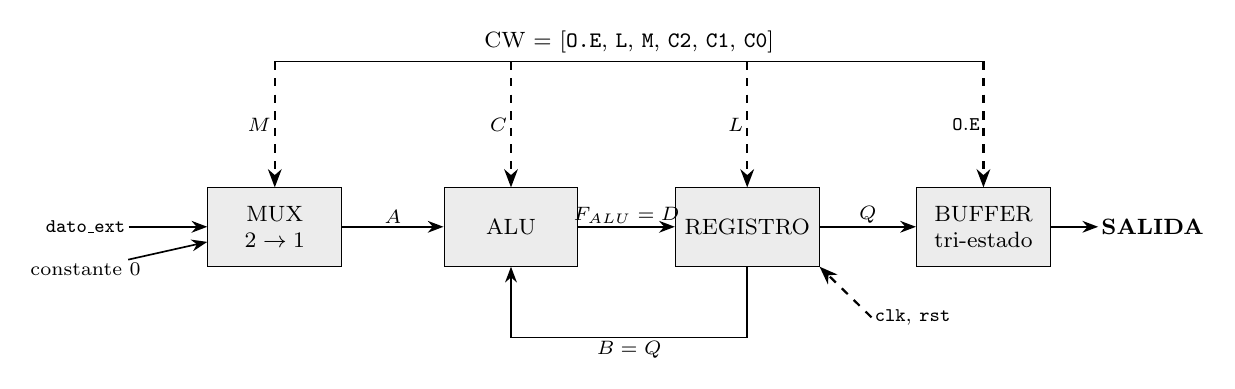
\begin{tikzpicture}[
      >=Stealth,
      blk/.style={draw, fill=gray!15, minimum width=17mm, minimum height=10mm,
                  align=center, font=\footnotesize},
      wire/.style={->, semithick},
      cwire/.style={->, thick, dashed},
      lab/.style={font=\scriptsize, inner sep=1pt}
    ]
    % ---- cadena de datos
    \node[blk] (mux) at (0,0)   {MUX\\ $2\to1$};
    \node[blk] (alu) at (3,0)   {ALU};
    \node[blk] (reg) at (6,0)   {REGISTRO};
    \node[blk] (buf) at (9,0)   {BUFFER\\ tri-estado};
    \node[lab, right=6mm of buf, font=\footnotesize\bfseries] (sal) {SALIDA};

    \node[lab, left=10mm of mux] (dext) {\texttt{dato\_ext}};
    \node[lab, below=3mm of dext] (cero) {constante $0$};

    \draw[wire] (dext) -- (mux);
    \draw[wire] (cero) -- (mux);
    \draw[wire] (mux) -- node[lab, above] {$A$} (alu);
    \draw[wire] (alu) -- node[lab, above] {$F_{ALU}=D$} (reg);
    \draw[wire] (reg) -- node[lab, above] {$Q$} (buf);
    \draw[wire] (buf) -- (sal);

    % ---- realimentación Q -> B
    \draw[wire] (reg.south) -- ++(0,-9mm) -- node[lab, below] {$B=Q$}
                ++(-3,0) -- (alu.south);

    % ---- bus de control
    \draw[semithick] (0,2.1) -- (9,2.1);
    \node[lab, above=2pt] at (4.5,2.1)
      {\footnotesize CW $=$ [\texttt{O.E}, \texttt{L}, \texttt{M},
       \texttt{C2}, \texttt{C1}, \texttt{C0}]};
    \draw[cwire] (0,2.1) -- node[lab, left] {$M$}  (0,0.5);
    \draw[cwire] (3,2.1) -- node[lab, left] {$C$}  (3,0.5);
    \draw[cwire] (6,2.1) -- node[lab, left] {$L$}  (6,0.5);
    \draw[cwire] (9,2.1) -- node[lab, left]
      {$\mathtt{O.E}$} (9,0.5);

    % ---- clk y rst
    \node[lab] (clkrst) at (8.1,-1.15) {\texttt{clk}, \texttt{rst}};
    \draw[cwire] (clkrst.west) -- (reg.south east);
  \end{tikzpicture}}
  \caption{Arquitectura del Datapath 1 (elaboración propia a partir del
  material del curso): la palabra de control \texttt{cw} distribuye
  \texttt{O.E}, \texttt{L}, \texttt{M} y \texttt{C[2:0]}; la salida externa
  proviene del registro, nunca directamente de la ALU.}
  \label{fig:arquitectura}
\end{figure}

Las cuatro señales que intervienen son distintas y conviene no
confundirlas: $F_{ALU}$ es el resultado \emph{combinacional} de la ALU;
$D$ es la entrada del registro (en este diseño, el mismo cable que
$F_{ALU}$); $Q$ es el valor \emph{secuencial} almacenado, que cambia
únicamente en el flanco de reloj; y \texttt{salida} es el valor de $Q$
visible cuando \texttt{O.E}~$=1$. En forma compacta:

\begin{align*}
  A          &= \texttt{M} \mathbin{?} \texttt{dato\_ext} : 0,
    & \texttt{salida} &= \texttt{O.E} \mathbin{?} Q : \texttt{Z}, \\
  B          &= Q, &
  F_{ALU}    &= \mathrm{ALU}(A, B, C), \\
  D          &= F_{ALU}, &
  Q^{+}      &= \begin{cases}
      0   & \text{si \texttt{rst} $=1$},\\
      D   & \text{si \texttt{rst} $=0$ y \texttt{L} $=1$},\\
      Q   & \text{en otro caso},
    \end{cases}
\end{align*}

\noindent siendo $Q^{+}$ el valor que adopta el registro en cada flanco de
subida de \texttt{clk} (el reinicio tiene prioridad sobre la carga). De
esta ecuación se sigue una consecuencia temporal importante, verificada en
simulación (§\ref{sec:resultados}): con \texttt{L}~$=0$ el registro
conserva su valor y \texttt{salida} muestra el valor \emph{anterior},
aunque $F_{ALU}$ cambie por efecto de $A$, $B$ o $C$. La salida externa
sale del registro, no de la ALU.

El reinicio síncrono no aparece en la fotografía, pero es necesaria: sin
ella, $B$ no puede garantizarse en cero y la única vía de cargar
\texttt{dato\_ext} en el registro sería sumar con $B=0$ (§\ref{sec:alu-op}).
Se optó por \texttt{rst} síncrono con prioridad sobre \texttt{L}, patrón ya
usado en los registros del resto del proyecto.

\subsection{Módulos VHDL}
\label{sec:modulos}

Los modelos siguen las convenciones del proyecto: VHDL-2008
conservador~\cite{ieee1076_2008}, un fichero por entidad, paquetes
\texttt{ieee.std\_\-logic\_\-1164} y \texttt{ieee.numeric\_\-std}, y
combinación
de los estilos de descripción: \emph{dataflow} para el MUX y la ALU,
\emph{comportamental} para el registro y el buffer, y \emph{estructural}
para la integración~\cite{navabi1998vhdl}. Todos los módulos nuevos
declaran \texttt{generic ANCHO : natural := 8}, de modo que el ancho de los
buses es parametrizable y los mismos bancos de prueba pueden comprobar
anchos distintos~\cite{harris2015ddca}.

\begin{itemize}
  \item \texttt{mux\_entrada}: entradas \texttt{dato\_ext} y constante
    cero, selección \texttt{sel} (el campo \texttt{M} de la palabra de
    control, con polaridad \texttt{'1'}~$=$ dato externo, decisión de
    diseño) y salida \texttt{y}, el operando $A$.
  \item \texttt{alu}: entradas \texttt{a}, \texttt{b} y código
    \texttt{c} de 3~bits; salida \texttt{f}. Un proceso con
    \texttt{case} implementa las tres operaciones de la
    §\ref{sec:alu-op} y devuelve cero para los códigos reservados.
  \item \texttt{registro}: entradas \texttt{clk}, \texttt{rst}, \texttt{l}
    y dato \texttt{d}; salida \texttt{q}. El proceso de carga con
    prioridad de reinicio es el siguiente (extracto de
    \texttt{registro.vhd}, código completo en el Apéndice):

\begin{lstlisting}[caption={\texttt{registro.vhd} --- proceso de carga con
  prioridad de reinicio}, label=lst:registro, numbers=left]
process (clk)
begin
    if rising_edge(clk) then
        if rst = '1' then
            contenido <= (others => '0');
        elsif l = '1' then
            contenido <= d;
        end if;
    end if;
end process;
\end{lstlisting}

  \item \texttt{buffer\_salida}: entradas \texttt{d\_in} y \texttt{oe};
    salida \texttt{y} con asignación condicional:
    \texttt{y <= d\_in when oe = '1' else (others => 'Z')}.
  \item \texttt{datapath}: integración \emph{estructural} que instancia
    los cuatro módulos por componentes ---de modo que el análisis del
    conjunto no depende del orden de los ficheros---, desempaqueta la
    palabra de control (\texttt{cw(5)}=\texttt{oe}, \texttt{cw(4)}=\texttt{l},
    \texttt{cw(3)}=\texttt{m}, \texttt{cw(2~downto~0)}=\texttt{c}),
    realimenta \texttt{q} al operando \texttt{b} y declara además dos
    salidas de observación, \texttt{f\_alu} y \texttt{q\_reg}, que
    permiten inspeccionar el resultado combinacional y el valor
    almacenado en los bancos de prueba y en las capturas de ondas sin
    formar parte de la salida externa.
\end{itemize}

\subsection{Palabra de control y operaciones de la ALU}
\label{sec:alu-op}

La señal \texttt{cw} tiene 6~bits y su formato, de más significativo a
menos, es \texttt{[O.E, L, M, C2, C1, C0]}
(Tabla~\ref{tab:palabra-control}). Los
campos \texttt{O.E}, \texttt{L} y el triplete \texttt{c[0:2]} están
tomados del material del curso; la polaridad de \texttt{M} y la
correspondencia bit a bit de los campos con \texttt{cw} son decisiones de
diseño del equipo.

\begin{table}[t]
  \centering
  \caption{Formato de la palabra de control \texttt{cw} (6~bits, de MSB a
  LSB).}
  \label{tab:palabra-control}
  \footnotesize
  \begin{tabular}{clll}
    \hline
    Bits & Campo & Acción & Origen \\
    \hline
    \texttt{cw[5]} & \texttt{O.E} & habilita la salida (desde $Q$) &
      foto (\texttt{O.E.}) \\
    \texttt{cw[4]} & \texttt{L}   & carga del registro (flanco de
      \texttt{clk}) & foto (nombre provis.) \\
    \texttt{cw[3]} & \texttt{M}   & MUX: \texttt{1}=\texttt{dato\_ext},
      \texttt{0}=cero & decisión \\
    \texttt{cw[2:0]} & \texttt{C2 C1 C0} & operación de la ALU &
      foto (\texttt{c[0:2]}) \\
    \hline
  \end{tabular}
\end{table}

La Tabla~\ref{tab:alu} resume las operaciones de la ALU. Las
\emph{expresiones} ($n+x$, $2n+x$, $n+1$) provienen del material del
curso; la \emph{codificación binaria} de la columna $C$ es una propuesta
explícita y provisional del equipo, acordada para poder implementar y
verificar el diseño: la codificación original del profesor no se pudo leer
en la fotografía. Los códigos \texttt{011}--\texttt{111} quedan
reservados, y se les asigna salida cero como valor por defecto inocuo
hasta contar con evidencia de su significado real.

\begin{table}[t]
  \centering
  \caption{Operaciones de la ALU: expresiones del material del curso y
  codificación binaria propuesta (provisional) por el equipo.}
  \label{tab:alu}
  \footnotesize
  \begin{tabular}{ccccl}
    \hline
    $C$ ($c_2c_1c_0$) & Nombre & Ecuación & Usa $A$ &
      Con $A=x$, $B=n$ \\
    \hline
    \texttt{000} & suma           & $F = A + B$          & sí & $n + x$ \\
    \texttt{001} & doble y suma   & $F = (B \ll 1) + A$  & sí & $2n + x$ \\
    \texttt{010} & incremento     & $F = B + 1$          & no & $n + 1$ \\
    \texttt{011}--\texttt{111} & reservado & $F = 0$ (propuesta) & --- & --- \\
    \hline
  \end{tabular}
\end{table}

La notación $n$ y $x$ del material de clases se corresponde con los
operandos del circuito: $n$ es el contenido actual del registro, es decir,
el operando $B$; $x$ es el valor externo presente en \texttt{dato\_ext}
cuando \texttt{M}~$=1$, es decir, el operando $A$ tras el MUX. Con esa
compatibilidad, las operaciones pedidas se obtienen así: $n+x$ con
\texttt{000} y \texttt{M}~$=1$; $2n+x$ con \texttt{001} y
\texttt{M}~$=1$, usando el desplazamiento lógico a la izquierda de un bit
de $B$ \emph{dentro} de la ALU; $n+1$ con \texttt{010}, operación que
ignora $A$ y por eso hace irrelevante \texttt{M}; y la carga directa de
$x$ en el registro se consigue con un \texttt{rst} previo ($B=0$) y
\texttt{000} con \texttt{M}~$=1$, de modo que $F=x+0=x$. Como limitación
documentada, con solo estas tres operaciones no es posible cargar $A$ en
un registro cuyo $B$ sea distinto de cero: por eso el reinicio es
necesario.

\subsection{Decisiones de diseño y limitaciones}
\label{sec:decisiones}

\begin{itemize}
  \item \textbf{Ancho parametrizable}: la fotografía no permite leer el
    ancho de los buses; se adopta \texttt{ANCHO := 8} como valor por
    defecto y todos los bancos de prueba trabajan también con anchos
    distintos (por ejemplo, 4~bits) para demostrar la parametrización.
  \item \textbf{Sin banderas}: no se modelan acarreo ni indicador de
    cero. Toda la aritmética es módulo $2^{\texttt{ANCHO}}$ y los
    desbordamientos son silenciosos: con 8~bits, doblar sin pérdida
    exige $n \le 127$, y $2n+x$ sin envoltura exige $2n+x \le 255$.
    Estos límites se caracterizan empíricamente en la
    Sección~\ref{sec:resultados}.
  \item \textbf{Sin FSM, sin shifter externo}: únicamente los módulos del
    esquema del curso más \texttt{clk} y \texttt{rst}.
  \item \textbf{Solo simulación}: el GHDL empleado usa el backend
    \texttt{mcode}, que no ofrece síntesis; no se afirma por tanto
    sintetizabilidad, únicamente comportamiento simulado~\cite{ghdl-docs}.
\end{itemize}

% ============================================================
% 3. PROPUESTA EXPERIMENTAL  (1 hoja)
% ============================================================
\section{Propuesta Experimental}
\label{sec:propuesta}

La metodología sigue un flujo descendente: de la especificación de la
§\ref{sec:diseno} se pasó a los modelos VHDL-2008, después a la
integración estructural y, en paralelo, a los bancos de prueba; la
verificación se hizo por simulación y el análisis de resultados por
inspección de ondas. Los modelos combinan los estilos \emph{dataflow},
\emph{comportamental} y \emph{estructural}~\cite{navabi1998vhdl} y sus
procesos siguen las sentencias secuenciales del lenguaje~\cite{ashenden2008vhdl},
con un estilo de diseño y de entidades consistente con el de los textos de
referencia del curso~\cite{harris2015ddca,ieee1076_2008}.

Las herramientas de simulación son GHDL~\cite{ghdl-docs}, invocado con el
estándar \texttt{--std=08} y volcado de ondas a formato VCD, y
GTKWave~\cite{gtkwave-docs} para la inspección de las ondas y la
exportación de capturas mediante scripts Tcl. La ejecución se apoya en los
scripts oficiales del repositorio: \texttt{vhdl-analizar} analiza las
fuentes, \texttt{vhdl-sim} analiza, elabora y ejecuta cada banco de
prueba, y \texttt{latexbuild} compila este informe en formato Springer
(llncs).

Se definieron cinco bancos de prueba autochequeados, uno por módulo y uno
de integración:

\begin{itemize}
  \item \texttt{tb\_mux\_entrada}: comprueba todas las selecciones del MUX
    con el genérico \texttt{ANCHO} igual a 8 y a 4~bits.
  \item \texttt{tb\_registro}: verifica el reinicio, la carga con
    \texttt{L} y la retención cuando \texttt{L}~$=0$.
  \item \texttt{tb\_buffer\_salida}: comprueba que con \texttt{oe}~$=1$
    propaga el dato y con \texttt{oe}~$=0$ entrega alta impedancia.
  \item \texttt{tb\_alu}: 27~comprobaciones sobre las tres operaciones
    (incluidos operandos nulos y máximos), los desbordamientos
    ($200+100$ sobre 8~bits, $200 \ll 1$ con pérdida del bit más
    significativo, $255+1$ envolviendo a cero), los códigos reservados y
    un segundo ejemplo con \texttt{ANCHO} igual a 4~bits.
  \item \texttt{tb\_datapath}: aplica las cinco palabras de control
    verificadas, reproduce el ejemplo completo de tres ciclos
    ($x=5$ con reinicio inicial) y ejecuta la prueba discriminante
    \texttt{L}~$=0$: con \texttt{CW = 100010} la ALU calcula $n+1$,
    pero la salida externa debe seguir siendo $n$.
\end{itemize}

Cada banco de prueba termina siempre con un mensaje de éxito
(\texttt{tb\_...: OK}) y falla con \texttt{assert ... severity failure}
ante cualquier desviación respecto al valor esperado. El pulso de reloj se
genera dentro del proceso estimulador ---patrón de todos los bancos de
prueba del proyecto, ya que \texttt{vhdl-sim} no impone un límite
de tiempo---, de modo que toda simulación termina de forma
determinista. Además, la integración continua del repositorio ejecuta la
batería completa de \texttt{tb\_*.vhd} en cada cambio.

El procedimiento de evaluación, repetido para cada experimento, fue:
(1)~analizar la unidad con el script \texttt{vhdl-analizar};
(2)~ejecutar el banco de prueba con \texttt{vhdl-sim} y comprobar en
consola que termina con \texttt{OK} y sin errores de GHDL;
(3)~volcar el VCD resultante;
(4)~capturar las ondas relevantes a PNG con GTKWave; y (5)~contrastar los
valores esperados y observados de las señales. Criterio de éxito: los
cinco bancos terminan con \texttt{OK} y ninguna aserción se dispara. Los
casos en que el resultado aritmético difiere del valor matemático exacto
por envoltura módulo $2^{\texttt{ANCHO}}$ no se consideran fallos, sino
comportamiento documentado en la Sección~\ref{sec:decisiones} y analizado
en la Sección~\ref{sec:resultados}.

% ============================================================
% 4. SIMULACIONES DE VHDL  (capturas de los módulos más importantes)
% ============================================================
\section{Simulaciones de VHDL}
\label{sec:simulaciones}

Capturas de los módulos más importantes (máximo 2 hojas). Exporta las ondas
de \texttt{vhdl/datapath-1/salidas/*.vcd} a PNG en \texttt{figuras/}.

% Descomenta el bloque cuando exista la captura en figuras/
% \begin{figure}[t]
%   \centering
%   \includegraphics[width=0.9\textwidth]{figuras/captura_modulo.png}
%   \caption{Simulación de <módulo>: descripción breve de lo que se observa.}
%   \label{fig:captura}
% \end{figure}

% ============================================================
% 5. RESULTADOS  (3–5 cuartillas)
% ============================================================
\section{Resultados}
\label{sec:resultados}

Análisis de las simulaciones: tablas comparativas, tiempos, comportamiento
observado, cumplimiento de las pruebas (assert). Interpretación crítica.
(3--5 cuartillas.)

% ============================================================
% 6. CONCLUSIONES  (1 cuartilla)
% ============================================================
\section{Conclusiones}
\label{sec:conclusiones}

Cierre: logros frente a los objetivos, limitaciones y trabajo futuro.
(1 cuartilla.)

% ============================================================
% REFERENCIAS  (>= 15 — indicar exactamente dónde aparece el texto)
% ============================================================
% IMPORTANTE: cada referencia debe permitir ubicar exactamente dónde
% aparece el texto sugerido (capítulo/§/página, o URL + fecha de consulta).
% Anota la ubicación en un comentario % justo debajo de la entrada.
\bibliographystyle{splncs04}
\bibliography{referencias}

% ============================================================
% APÉNDICE — CÓDIGO VHDL
% ============================================================
\appendix
\section{Código VHDL}
\label{app:codigo}

Código completo de los módulos de la unidad (copiado de
\texttt{vhdl/datapath\-1/src/}). Usa \texttt{lstlisting}:

% Sustituye por el código real de cada módulo de la unidad.
% \begin{lstlisting}[caption={sumador.vhd --- <descripción>}, label=lst:sumador]
% library ieee;
% use ieee.std_logic_1164.all;
% use ieee.numeric_std.all;
% ...
% \end{lstlisting}

\end{document}
